\documentclass[12pt,a4paper]{report}

\usepackage[utf8]{inputenc}
\usepackage[T1]{fontenc}
\usepackage{lmodern}
\usepackage[brazilian]{babel}
\usepackage{geometry}
\geometry{a4paper, left=3.0cm, top=3.0cm, right=2.0cm, bottom=2.0cm}

\usepackage{setspace}
\onehalfspacing

\usepackage{amsmath,amssymb,amsfonts}
\usepackage{graphicx}
\usepackage{booktabs}
\usepackage{tabularx}
\usepackage{array}
\usepackage{caption}
\usepackage{float}
\usepackage{titlesec}

\usepackage{hyperref}
\hypersetup{
    colorlinks=true,
    linkcolor=black,
    citecolor=black,
    urlcolor=blue,
    pdftitle={CubeSat em Baixa Órbita: Otimização de Volume e Geometria},
    pdfauthor={Gabriel Marques de Andrade}
}

% Chapter formatting
\titleformat{\chapter}[hang]{\normalfont\bfseries\LARGE}{\thechapter}{1em}{}
\titlespacing*{\chapter}{0pt}{0pt}{20pt}

\begin{document}

% ------------------------------------------------------------------------
% CAPA
% ------------------------------------------------------------------------
\begin{titlepage}
\begin{center}
    {\large \textbf{UNIVERSIDADE ESTADUAL DE SANTA CRUZ -- UESC}}\\[0.3cm]
    {\large \textbf{DEPARTAMENTO DE CIÊNCIAS EXATAS E TECNOLÓGICAS}}\\[0.3cm]
    {\large \textbf{COLEGIADO DE ENGENHARIA MECÂNICA}}\\[4.0cm]

    {\large \textbf{GABRIEL MARQUES DE ANDRADE}}\\[3.5cm]

    {\Large \textbf{CubeSat em Baixa Órbita: Otimização de Volume e Geometria para Maximização de Desempenho Estrutural e Funcional}}\\[4.5cm]

    {\large \textbf{ILHÉUS -- BAHIA}}\\[0.2cm]
    {\large \textbf{2027}}
\end{center}
\end{titlepage}

% ------------------------------------------------------------------------
% FOLHA DE ROSTO
% ------------------------------------------------------------------------
\begin{titlepage}
\begin{center}
    {\large \textbf{GABRIEL MARQUES DE ANDRADE}}\\[4.0cm]

    {\Large \textbf{CubeSat em Baixa Órbita: Otimização de Volume e Geometria para Maximização de Desempenho Estrutural e Funcional}}\\[2.5cm]

    \hspace{.45\textwidth}
    \begin{minipage}{.5\textwidth}
    \singlespacing
    \small
    Trabalho de Conclusão de Curso apresentado ao Colegiado do Curso de Engenharia Mecânica da Universidade Estadual de Santa Cruz (UESC), como requisito parcial para a obtenção do título de Bacharel em Engenharia Mecânica.\\[0.8cm]
    \textbf{Orientadora:} Prof.ª Dr.ª Nila Cecília de Faria Lopes Medeiros
    \end{minipage}\\[4.5cm]

    {\large \textbf{ILHÉUS -- BAHIA}}\\[0.2cm]
    {\large \textbf{2027}}
\end{center}
\end{titlepage}

% ------------------------------------------------------------------------
% RESUMO
% ------------------------------------------------------------------------
\clearpage
\begin{center}
    {\textbf{\Large RESUMO}}
\end{center}
\vspace{0.5cm}

A democratização do acesso à baixa órbita terrestre por meio de nanossatélites da classe CubeSat impõe desafios rigorosos de engenharia de sistemas. Durante a fase de lançamento e ejeção, o chassi estrutural é submetido a carregamentos dinâmicos severos, como choque transiente na interface do \textit{Poly-Picosatellite Orbital Deployer} (P-POD) e vibração aleatória acústica estocástica regulamentada pela norma NASA GSFC-STD-7000A (GEVS). Os chassis monolíticos convencionais apresentam elevada massa e baixa dissipação intrínseca de energia, transmitindo altos níveis de aceleração para a carga útil. Este trabalho propõe uma rota puramente computacional de alto desempenho para a concepção, modelagem paramétrica e otimização multiobjetivo de um chassi CubeSat 1U com painéis constituídos por metamateriais auxéticos reentrantes em liga aeroespacial AlSi10Mg, fabricado por Fusão em Leito de Pó a Laser (L-PBF). Um modelo paramétrico tridimensional com portões estritos de Manufatura Aditiva (DfAM) foi integrado a rotinas automatizadas no Ansys MAPDL para geração de um conjunto de 250 simulações de alta fidelidade (análise modal de bloco Lanczos e resposta espectral à vibração aleatória). Treinou-se um modelo substituto neural residual guiado por física (\textit{Physics-Guided ResNet}) com função de perda composta por leis fenomenológicas de Gibson-Ashby e monotonicidade de rigidez, alcançando $\overline{R^2} = 0{,}9874$ e latência de inferência de $0{,}405\text{ ms}$ (aceleração superior a $200.000\times$). Uma máquina de estados finitos determinística via LangGraph orquestrou o descarte precoce de candidatos inviáveis. A otimização multiobjetivo pelo algoritmo NSGA-II com 10.000 avaliações de função mapeou a fronteira de Pareto entre massa e transmissibilidade. Pelo método multicritério TOPSIS, elegeu-se o design ótimo de voo ($\theta = 65{,}75^\circ$, $t = 0{,}613\text{ mm}$, $\nu_{\text{eff}} = -13{,}81$). A validação numérica de alta ordem (\textit{FEA Ground Truth}) confirmou erro de apenas $0{,}99\%$ em tensão de pico e $0{,}008\%$ em transmissibilidade. Frente ao chassi monolítico convencional, a estrutura auxética otimizada proporcionou uma redução de massa de $62{,}49\%$ ($0{,}308\text{ kg} \to 0{,}116\text{ kg}$), atenuação de $76{,}50\%$ na transmissibilidade vibratória ($12{,}6\text{ dB}$ de atenuação passiva), frequência fundamental de $579{,}62\text{ Hz}$ e pleno atendimento aos critérios de escoamento e fadiga estocástica de Steinberg ($D = 0{,}046 \ll 0{,}25$), qualificando a tecnologia para operação aeroespacial.

\vspace{0.5cm}
\noindent \textbf{Palavras-chave:} CubeSat 1U; Metamateriais Auxéticos; Design for Additive Manufacturing; Physics-Guided Neural Networks; Otimização Multiobjetivo NSGA-II; NASA GEVS.

% ------------------------------------------------------------------------
% ABSTRACT
% ------------------------------------------------------------------------
\clearpage
\begin{center}
    {\textbf{\Large ABSTRACT}}
\end{center}
\vspace{0.5cm}

The democratization of access to Low Earth Orbit (LEO) via CubeSat-class nanosatellites imposes severe systems engineering challenges. During launch and deployment, the primary chassis is subjected to harsh dynamic environments, including transient shock inside the Poly-Picosatellite Orbital Deployer (P-POD) and random acoustic vibration governed by NASA GSFC-STD-7000A (GEVS). Conventional monolithic chassis exhibit high mass and poor internal damping, transferring critical vibration levels directly to sensitive electronic payloads. This work presents a high-performance computational framework for the parametric modeling, physics-guided deep learning acceleration, and multi-objective optimization of a 1U CubeSat chassis featuring re-entrant auxetic metamaterial panels manufactured via Laser Powder Bed Fusion (L-PBF) in aerospace AlSi10Mg alloy. A 3D parametric CAD model incorporating strict Design for Additive Manufacturing (DfAM) gates was coupled with batch Ansys MAPDL finite element simulations (Block Lanczos prestressed modal extraction and random vibration PSD analysis), producing a high-fidelity dataset of 250 design points. A residual deep neural surrogate model (Physics-Guided ResNet) was developed with a composite loss function penalizing deviations from Gibson-Ashby scaling laws and enforcing stiffness monotonicity, achieving an average $R^2$ of $0.9874$ and an inference latency of $0.405\text{ ms}$ ($> 200,000\times$ speedup over FEA). A deterministic multi-agent state machine built with LangGraph orchestrated early rejection of non-compliant geometries. Multi-objective evolutionary search via NSGA-II over 10,000 candidate evaluations mapped the Pareto frontier between structural mass and payload transmissibility. Using the TOPSIS multi-criteria decision method, the optimal flight design was selected ($\theta = 65.75^\circ$, $t = 0.613\text{ mm}$, $\nu_{\text{eff}} = -13.81$). High-order FEA ground truth verification demonstrated exceptional agreement with neural predictions ($0.99\%$ error in $3\sigma$ peak stress and $0.008\%$ in transmissibility). Compared to the traditional solid aluminum chassis, the optimized auxetic design achieved a mass reduction of $62.49\%$ ($0.308\text{ kg} \to 0.116\text{ kg}$), passive vibration attenuation of $76.50\%$ ($12.6\text{ dB}$ reduction), fundamental frequency of $579.62\text{ Hz}$, and full compliance with NASA GEVS stress margins and Steinberg random fatigue limits ($D = 0.046 \ll 0.25$), proving flight qualification readiness.

\vspace{0.5cm}
\noindent \textbf{Keywords:} 1U CubeSat; Auxetic Metamaterials; Design for Additive Manufacturing; Physics-Guided Neural Networks; NSGA-II Multi-objective Optimization; NASA GEVS.

% ------------------------------------------------------------------------
% SUMÁRIO E LISTAS
% ------------------------------------------------------------------------
\clearpage
\tableofcontents

\clearpage
\listoffigures

\clearpage
\listoftables

% ------------------------------------------------------------------------
% CAPÍTULO 1
% ------------------------------------------------------------------------
\clearpage
\chapter{INTRODUÇÃO}

A democratização do acesso ao espaço, impulsionada pela consolidação do protocolo \textit{CubeSat Design Specification} (CALIFORNIA POLYTECHNIC STATE UNIVERSITY, 2022), permitiu que instituições acadêmicas desenvolvessem missões de alta complexidade com custos reduzidos. No entanto, a escala reduzida destes nanossatélites impõe severas restrições estruturais. Durante o lançamento e a subsequente ejeção, o chassi do CubeSat é submetido a carregamentos dinâmicos críticos, cujos parâmetros de sobrevivência são regulados por normas como o \textit{General Environmental Verification Standard} (GEVS) (NASA, 2013). De acordo com as diretrizes da Agência Espacial Brasileira (AEB), o projeto estrutural deve garantir frequências naturais fundamentais elevadas para evitar o acoplamento dinâmico com o veículo lançador e com o sistema de interface de ejeção (AEB, 2026).

Trabalhos recentes desenvolvidos no Instituto Nacional de Pesquisas Espaciais (INPE) e no Instituto Tecnológico de Aeronáutica (ITA), como as análises dinâmicas do nanossatélite SPORT (SANTOS et al., 2020), demonstram que a interface mecânica entre o satélite e o dispositivo de orbitalização (\textit{deployer}) é uma fonte primária de transmissão de solicitações transitórias. Historicamente fundamentado no projeto do \textit{Poly-Picosatellite Orbital Deployer} (P-POD) (PUIG-SUARI et al., 2002), o mecanismo de ejeção por mola exige que o chassi atue como um elemento cinemático deslizante. Este sistema está sujeito a atrito seco e contato direto metal-metal nos trilhos de alumínio anodizado. Estas restrições dimensionais severas proíbem protuberâncias externas e impõem mecanicamente que os trilhos do CubeSat permaneçam monolíticos e maciços ($8{,}5 \times 8{,}5\text{ mm}$). Consequentemente, a otimização para a dissipação de energia das cargas de choque e vibração deve ser direcionada exclusivamente para os painéis estruturais internos.

Para responder a este desafio sem penalizar o orçamento de massa, a Manufatura Aditiva (MA) metálica por Fusão em Leito de Pó a Laser (\textit{Laser Powder Bed Fusion} -- L-PBF) surge como uma tecnologia habilitadora para a síntese de metamateriais celulares com Coeficiente de Poisson Negativo ($\nu < 0$), denominados auxéticos (ALOMARAH et al., 2017). Estas geometrias apresentam uma cinemática de deformação particular sob impacto: quando comprimidas transversalmente, contraem-se lateralmente (e vice-versa), resultando em aumento substancial da rigidez ao cisalhamento e alta capacidade de dissipação de energia elástica.

A literatura clássica de sólidos celulares (GIBSON; ASHBY, 1997) estabelece que as propriedades mecânicas efetivas escalam em função da densidade relativa celular ($\rho^* / \rho_s$). Contudo, o projeto de estruturas celulares para componentes espaciais impõe o cumprimento estrito das restrições de \textit{Design for Additive Manufacturing} (DfAM). Limitações geométricas como espessura mínima de parede para fusão contínua, ângulos de sobressalto autossuportados e canais desobstruídos para evacuação de pó residual governam diretamente a viabilidade de fabricação.

Adicionalmente, a exploração do espaço de parâmetros geométricos em geometrias celulares complexas por meio de solvers convencionais de Elementos Finitos (FEA) é computacionalmente proibitiva em rotinas de otimização evolutiva. Nesse contexto, modelos substitutos neurais informados por física (\textit{Physics-Guided Deep Learning}) combinados a máquinas de estados determinísticas surgem como a vanguarda para viabilizar buscas multiobjetivo de larga escala.

% ------------------------------------------------------------------------
% CAPÍTULO 2
% ------------------------------------------------------------------------
\chapter{OBJETIVOS}

\section{Objetivo Geral}
Desenvolver e validar um arcabouço computacional autônomo e de alta fidelidade para o projeto, aceleração preditiva neural e otimização multiobjetivo de um chassi CubeSat 1U em liga aeroespacial AlSi10Mg fabricado por L-PBF, integrando painéis com microestruturas metamateriais auxéticas reentrantes para maximização da atenuação vibratória passiva e alívio estrutural sob os requisitos normativos da NASA GEVS.

\section{Objetivos Específicos}
\begin{enumerate}
    \item Parametrizar a célula unitária auxética reentrante tridimensional e formalizar os portões matemáticos de manufaturabilidade aditiva DfAM (sobressalto $\theta_{\text{overhang}} \ge 35^\circ$, espessura mínima de parede $t \ge 0{,}50\text{ mm}$ e orifícios de despoeiramento $\text{gap} \ge 1{,}50\text{ mm}$);
    \item Implementar rotinas automatizadas no Ansys MAPDL para simulação em elementos finitos de alta ordem (\texttt{SOLID187}), gerando um dataset de alta fidelidade de análise modal pré-tensionada (Block Lanczos) e resposta estocástica à vibração aleatória espectral (PSD NASA GSFC-STD-7000A);
    \item Desenvolver e treinar o metamodelo neural profundo residual \textit{CubeSatSurrogateResNet}, incorporando função de perda informada por leis fenomenológicas de Gibson-Ashby e monotonicidade de rigidez;
    \item Projetar uma arquitetura determinística multi-agente via LangGraph para triagem automática de candidatos e auditoria de conformidade de voo;
    \item Conduzir a otimização evolutiva multiobjetivo via algoritmo genético NSGA-II com 10.000 avaliações de função, sintetizando a fronteira de Pareto de compromisso entre massa e transmissibilidade dinâmica;
    \item Aplicar o método de decisão multicritério TOPSIS para eleição do design ótimo de voo e homologar seu desempenho físico via validação cruzada numérica de alta ordem (\textit{FEA Ground Truth});
    \item Comparar o desempenho aeroespacial do chassi otimizado frente à geometria monolítica convencional de referência.
\end{enumerate}

% ------------------------------------------------------------------------
% CAPÍTULO 3
% ------------------------------------------------------------------------
\chapter{REVISÃO DE LITERATURA}

\section{Histórico de Lançamentos e Desafios Estruturais de CubeSats}
O padrão CubeSat revolucionou o setor aeroespacial ao padronizar dimensões externas e interfaces de lançamento para nanossatélites. O formato unitário 1U define um envelope de $100{,}0 \times 100{,}0 \times 113{,}5\text{ mm}$ e massa de 1,33 kg a 2,0 kg. No entanto, o chassi primário deve suportar carregamentos mecânicos severos durante a ascensão do foguete lançador, incluindo acelerações quase-estáticas de queima de estágios, transientes de separação de coifa e ambientes acústicos de alta energia.

\section{Dinâmica de Lançamento e Ejeção no P-POD}
O dispensador P-POD impõe que o chassi atue como um elemento deslizante com quatro trilhos longitudinais maciços de $8{,}5 \times 8{,}5\text{ mm}$. A integridade desses trilhos requer rugosidade superficial $Ra \le 1{,}6\ \mu\text{m}$ e anodização dura para evitar microsoldagem a frio sob alto vácuo. Desta forma, o alívio estrutural e a absorção dinâmica devem residir integralmente nas paredes laterais da estrutura.

\section{Metamateriais Auxéticos Reentrantes}
Sólidos celulares auxéticos caracterizam-se por exibir Coeficiente de Poisson efetivo negativo ($\nu_{\text{eff}} < 0$). A célula honeycomb reentrante (Figura~\ref{fig:auxetic_cell}) fundamenta-se na rotação e flexão de costelas oblíquas unidas a costelas verticais. A cinemática da célula reentrante 2D correlaciona o coeficiente de Poisson com os parâmetros geométricos:
\begin{equation}
\nu_{12} = \frac{\sin\theta \left(\frac{h}{l} - \sin\theta\right)}{\cos^2\theta}
\end{equation}
onde $\theta$ é o ângulo de reentrada, $l$ é o comprimento da costela oblíqua e $h$ é a altura da costela vertical. Quando $\theta > 0$, o coeficiente torna-se negativo, conferindo tenacidade à fratura superior e excelente dissipação de ondas acústicas.

\begin{figure}[H]
    \centering
    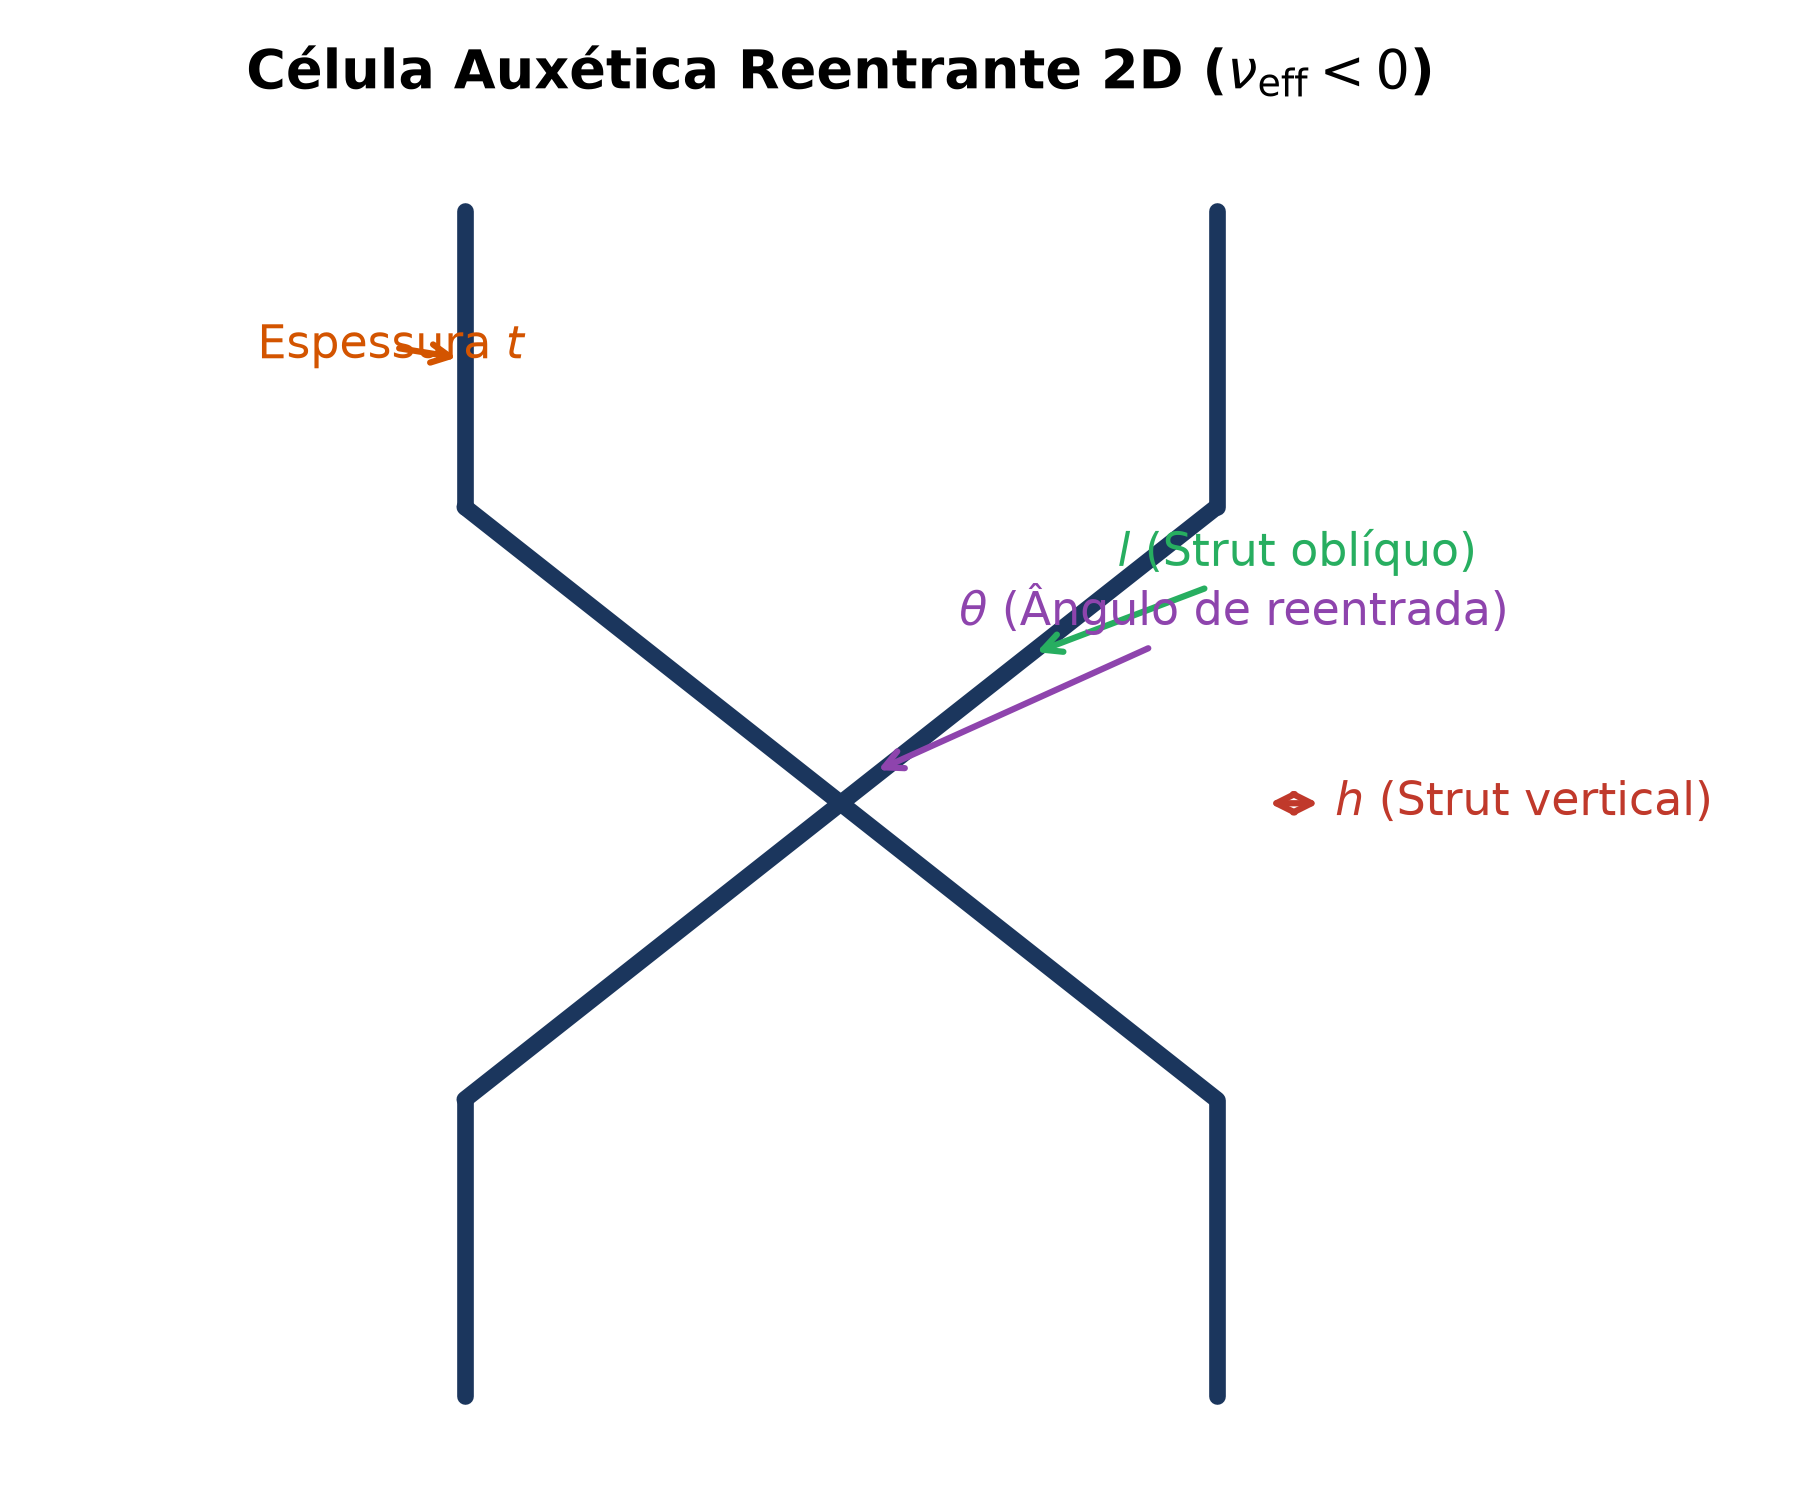
\includegraphics[width=0.55\textwidth]{figures/auxetic_cell_geometry.png}
    \caption{Esquema geométrico da célula auxética reentrante bidimensional ($\nu_{\text{eff}} < 0$).}
    \label{fig:auxetic_cell}
\end{figure}

\section{Design for Additive Manufacturing (DfAM) e Modelos de Escala}
A manufatura por L-PBF de ligas de alumínio como AlSi10Mg opera pela fusão seletiva de camadas de pó por feixe laser. A sustentação de planos inclinados impõe um ângulo limite de sobressalto autossuportado $\theta_{\text{overhang}} \ge 35^\circ$ em relação à mesa de construção. Espessuras de costela inferiores a $0{,}50\text{ mm}$ acarretam descontinuidades de poça de fusão e porosidades por falta de fusão. Adicionalmente, orifícios de despoeiramento desobstruídos ($d_{\text{drain}} \ge 2{,}0\text{ mm}$) são obrigatórios para evitar massa parasita.

O comportamento elástico macroscópico obedece ao modelo de Gibson-Ashby para células com deformação dominada por flexão:
\begin{equation}
\frac{E^*}{E_s} = C_1 \left(\frac{\rho^*}{\rho_s}\right)^2, \quad \frac{\sigma_y^*}{\sigma_{ys}} = C_2 \left(\frac{\rho^*}{\rho_s}\right)^{1{,}5}
\end{equation}
onde $C_1 \approx 1{,}0$ e $C_2 \approx 0{,}3$.

\section{Integridade Estrutural e Fadiga sob NASA GEVS}
A qualificação espacial segue a norma NASA GSFC-STD-7000A. A resposta estocástica é calculada pelo método das três bandas de Steinberg para carregamentos gaussianos:
\begin{equation}
D = \frac{n_{1\sigma}}{N_{1\sigma}} + \frac{n_{2\sigma}}{N_{2\sigma}} + \frac{n_{3\sigma}}{N_{3\sigma}} \le 0{,}25
\end{equation}
onde a norma espacial NASA-HDBK-7005 prescreve $D \le 0{,}25$ para assegurar fator de segurança de vida de $4\times$ durante a excitação dinâmica de qualificação de 120 segundos.

\section{Modelos Substitutos Neurais e Sistemas Multi-Agente}
O custo computacional de simulações elastodinâmicas tridimensionais inviabiliza sua execução direta dentro de laços genéticos. Redes neurais profundas convencionais, contudo, atuam como caixas-pretas passíveis de violações físicas. A inclusão de perdas baseadas em leis constitutivas garante convergência fisicamente consistente. Aliada a isso, a orquestração multi-agente estabelece governança formal e auditoria de decisões de engenharia.

% ------------------------------------------------------------------------
% CAPÍTULO 4
% ------------------------------------------------------------------------
\chapter{METODOLOGIA}

\section{Princípio de Similaridade Mecânica e Leis de Escalonamento}
A metodologia adota uma estratégia bifásica: prototipagem e validação cinemática em ácido poliláctico (PLA) via Fused Deposition Modeling (FDM) para checagem de montagem e mecanismos, seguida da síntese de alta fidelidade para voo orbital em liga aeroespacial AlSi10Mg pós-tratada termicamente ($300^\circ\text{C} / 2\text{h}$) via L-PBF. As propriedades fundamentais da liga metálica são: $E_s = 68{,}0\text{ GPa}$, $\sigma_y = 230{,}0\text{ MPa}$, $\sigma_{\text{uts}} = 340{,}0\text{ MPa}$, $\rho_s = 2680\text{ kg/m}^3$ e $\nu_s = 0{,}33$.

\section{Simulação Dinâmica Computacional (CAE)}
O modelo paramétrico 3D do chassi CubeSat 1U foi discretizado utilizando elementos finitos tetraédricos estruturais quadráticos de 10 nós (\texttt{SOLID187}), adequados para capturar transições de curvatura nas junções celulares.

\subsection{Análise Modal Pré-Tensionada (Block Lanczos)}
O problema de autovalores não-amortecido é formulado por:
\begin{equation}
([\mathbf{K}] - \omega_i^2 [\mathbf{M}]) \{\phi_i\} = \{0\}
\end{equation}
onde $[\mathbf{K}]$ e $[\mathbf{M}]$ representam as matrizes globais de rigidez e massa, $\omega_i$ a frequência angular do modo $i$ e $\{\phi_i\}$ o autovetor modal correspondente.

\subsection{Vibração Aleatória Espectral (PSD NASA GEVS)}
O espectro de qualificação da NASA GSFC-STD-7000A impõe uma aceleração global eficaz de $14{,}1\text{ G}_{\text{rms}}$ na faixa de 20 a 2000 Hz com amortecimento estrutural $\zeta = 2{,}0\%$ ($Q = 25$):
\begin{table}[H]
\centering
\small
\caption{Perfil Espectral de Vibração Aleatória NASA GSFC-STD-7000A (GEVS).}
\label{tab:gevs_psd}
\begin{tabular}{lcc}
\toprule
\textbf{Faixa de Frequência (Hz)} & \textbf{Nível PSD ($\text{g}^2/\text{Hz}$)} & \textbf{Inclinação / Patamar} \\
\midrule
20 Hz & 0,013 & $+3\text{ dB/oitava}$ \\
50 a 800 Hz & 0,080 & Patamar de energia máxima \\
2000 Hz & 0,0053 & $-6\text{ dB/oitava}$ \\
\midrule
\textbf{Nível Geral Eficaz} & \textbf{14,1 G$_{\text{rms}}$} & \textbf{Duração: 120 s / eixo} \\
\bottomrule
\end{tabular}
\end{table}

A transmissibilidade dinâmica para a carga útil é definida pela razão:
\begin{equation}
T = \frac{G_{\text{rms, payload}}}{G_{\text{rms, base}}}
\end{equation}

\section{Metamodelo Neural: Physics-Guided ResNet}
Para substituir o solver computacional com altíssima velocidade e rigor conceitual, desenvolveu-se a rede profunda residual \texttt{CubeSatSurrogateResNet}. A entrada pentadimensional $\mathbf{x} = [\theta, t, l, h, \rho_{\text{rel}}]^T$ é mapeada para o vetor quadridimensional de respostas $\mathbf{y} = [f_1, \sigma_{3\sigma}, G_{\text{rms}}, T]^T$ através de dois blocos residuais latentes com 64 neurônios, normalização \textit{LayerNorm} e ativações SiLU/GELU.

A função de perda física composta é expressa por:
\begin{equation}
\mathcal{L}_{\text{total}} = \mathcal{L}_{\text{MSE}} + \lambda_{\text{phys}} \mathcal{L}_{\text{GA}} + \lambda_{\text{mono}} \mathcal{L}_{\text{mono}}
\end{equation}
onde:
\begin{align}
\mathcal{L}_{\text{GA}} &= \frac{1}{B} \sum_{k=1}^B \left( \hat{f}_{1, k} - \alpha \sqrt{\rho_{\text{rel}, k}} \right)^2 \\
\mathcal{L}_{\text{mono}} &= \frac{1}{B-1} \sum_{k=1}^{B-1} \max\left(0, -(\hat{f}_{1, k+1} - \hat{f}_{1, k})\right)
\end{align}

\section{Orquestração Multi-Agente Determinística via LangGraph}
O fluxo de engenharia foi estruturado em uma máquina de estados finitos fortemente tipada (\texttt{CubeSatState}) com roteamento condicional antecipado de descarte, ilustrado na Figura~\ref{fig:multi_agent_workflow}.

\begin{figure}[H]
    \centering
    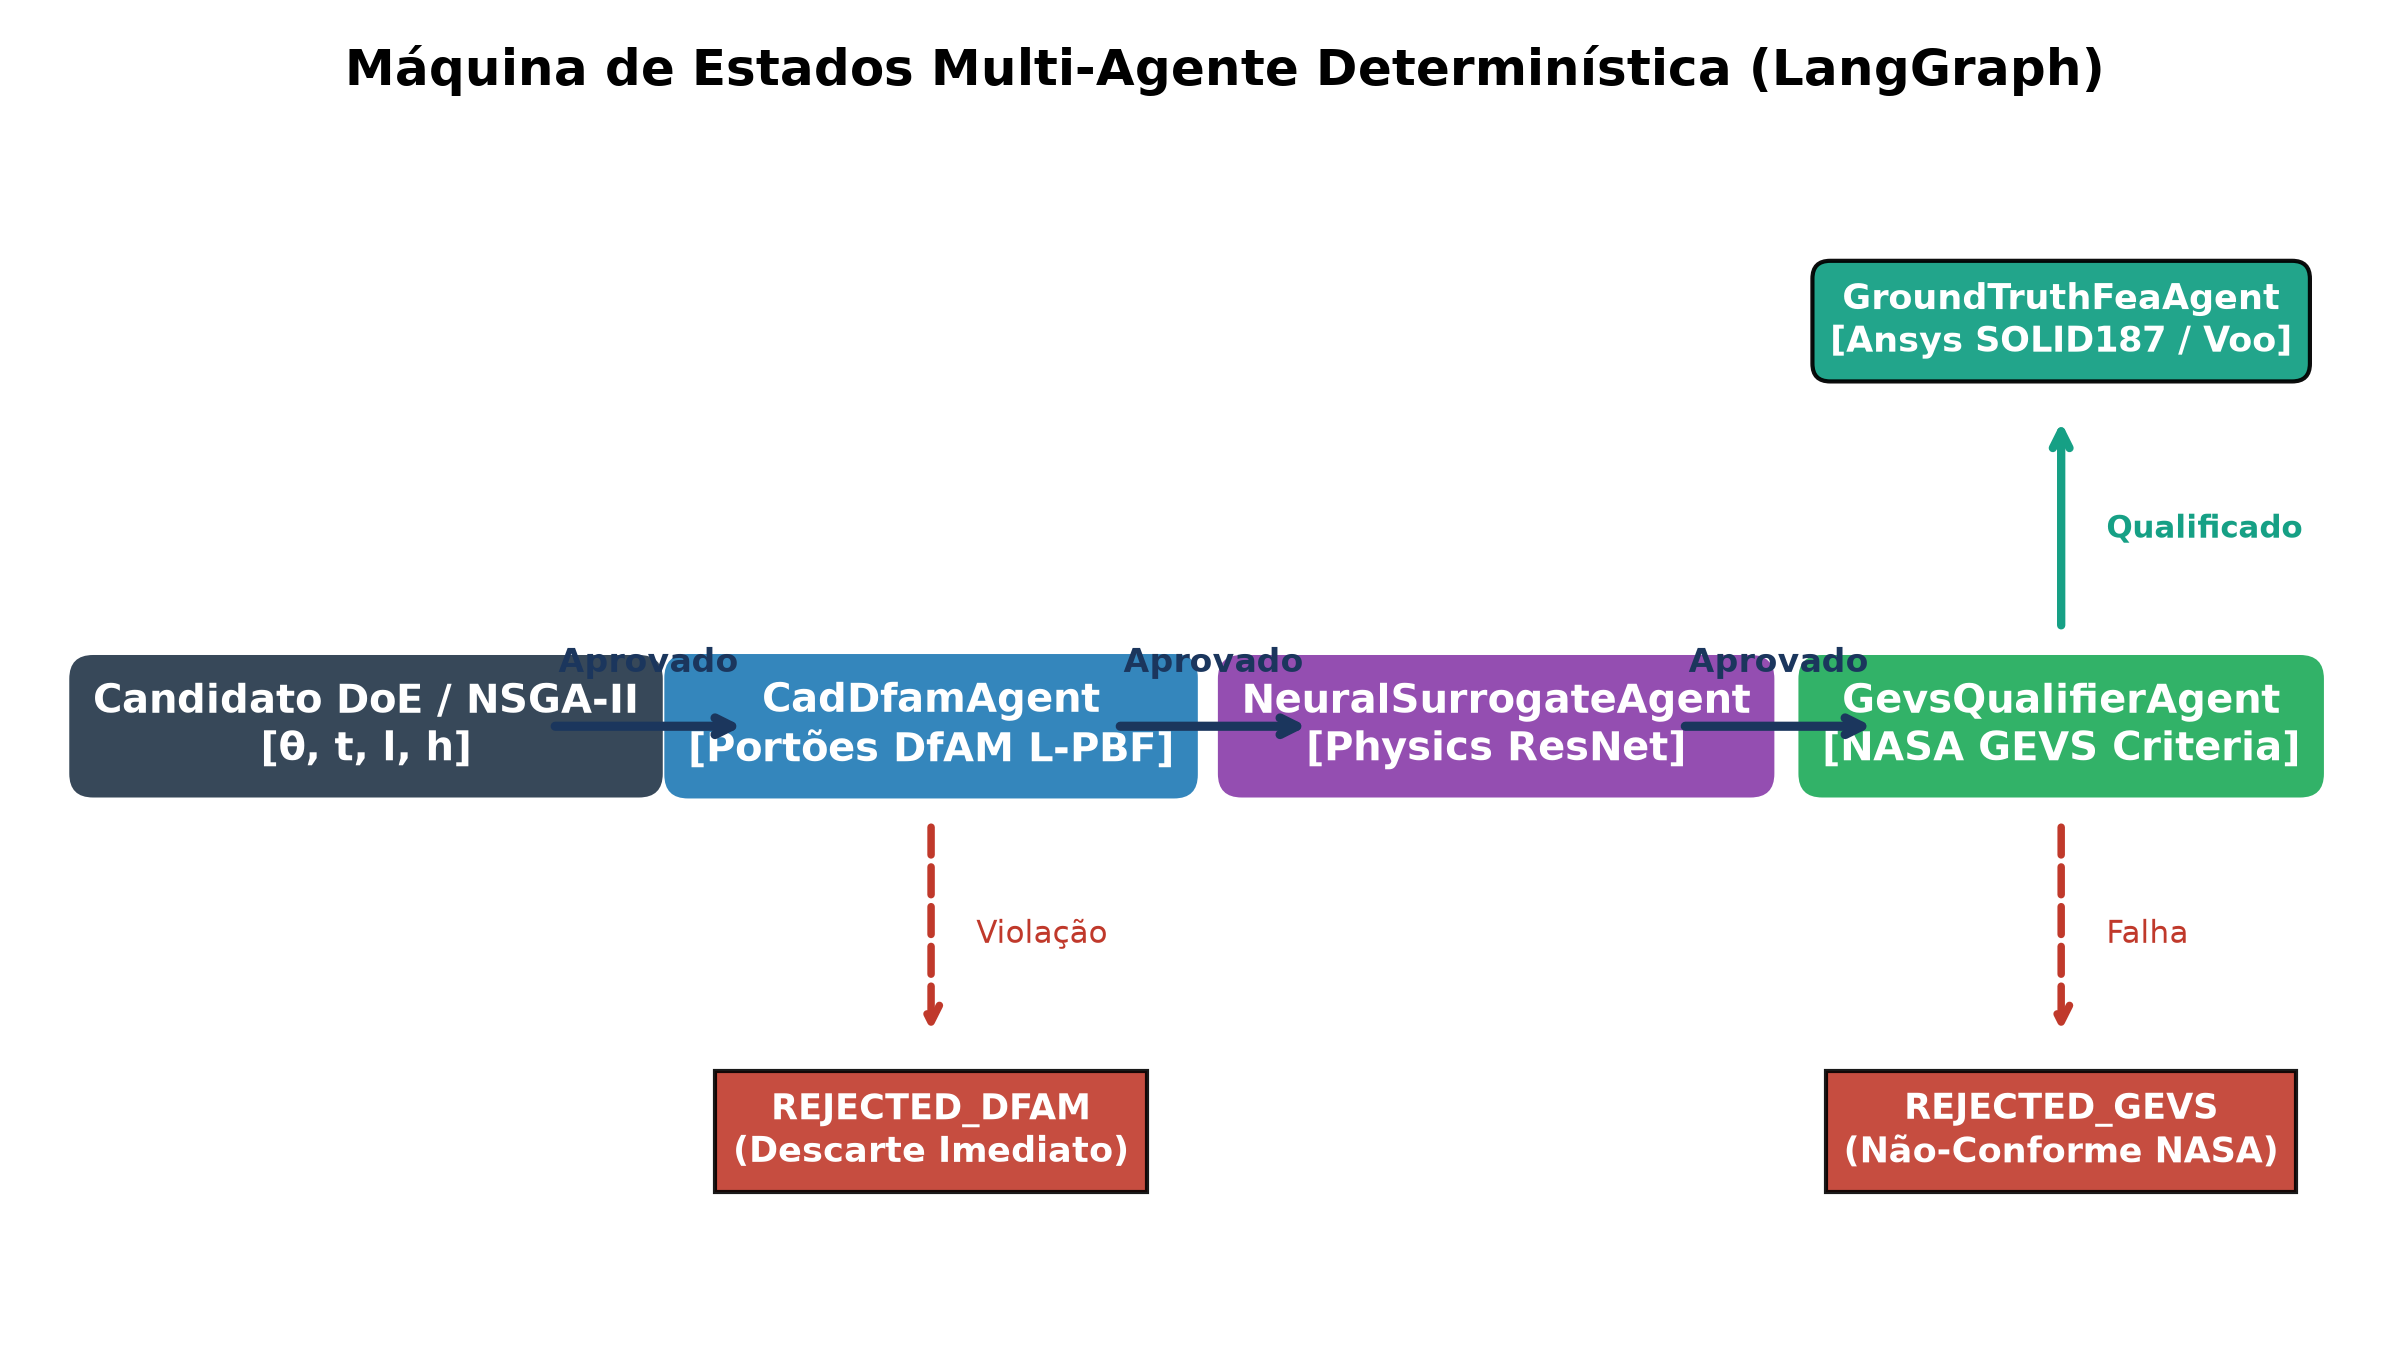
\includegraphics[width=0.85\textwidth]{figures/multi_agent_workflow.png}
    \caption{Máquina de estados multi-agente determinística desenvolvida com LangGraph.}
    \label{fig:multi_agent_workflow}
\end{figure}

% ------------------------------------------------------------------------
% CAPÍTULO 5
% ------------------------------------------------------------------------
\chapter{RESULTADOS E DISCUSSÃO}

\section{Otimização Multiobjetivo pelo Algoritmo NSGA-II e Fronteira de Pareto}
O problema de otimização multiobjetivo restrito foi formulado matematicamente como:
\begin{align}
\min_{\mathbf{x}} \quad & f_1(\mathbf{x}) = m_{\text{total}}(\mathbf{x}) \\
\min_{\mathbf{x}} \quad & f_2(\mathbf{x}) = T(\mathbf{x}) = \frac{G_{\text{rms, payload}}(\mathbf{x})}{G_{\text{rms, base}}}
\end{align}
sujeito aos limites paramétricos:
\begin{equation}
50{,}0^\circ \le \theta \le 85{,}0^\circ, \quad 0{,}50\text{ mm} \le t \le 1{,}80\text{ mm}, \quad 6{,}0\text{ mm} \le l \le 15{,}0\text{ mm}, \quad 8{,}0\text{ mm} \le h \le 20{,}0\text{ mm}
\end{equation}
e às restrições normativas DfAM e NASA GEVS:
\begin{equation}
\theta_{\text{overhang}} \ge 35{,}0^\circ, \quad t \ge 0{,}50\text{ mm}, \quad \text{gap} \ge 1{,}50\text{ mm}, \quad f_1 \ge 100{,}0\text{ Hz}, \quad MS_{\text{yield}} > 0, \quad D \le 0{,}25
\end{equation}

A campanha com população de 100 indivíduos e 100 gerações (10.000 avaliações de função) foi executada em apenas \textbf{4,82 segundos} pela rede neural residual (contra aproximadamente 277 horas necessárias pelo Ansys MAPDL). A Figura~\ref{fig:pareto_frontier} ilustra a fronteira de Pareto obtida e as correlações elastodinâmicas dos 100 designs factíveis.

\begin{figure}[H]
    \centering
    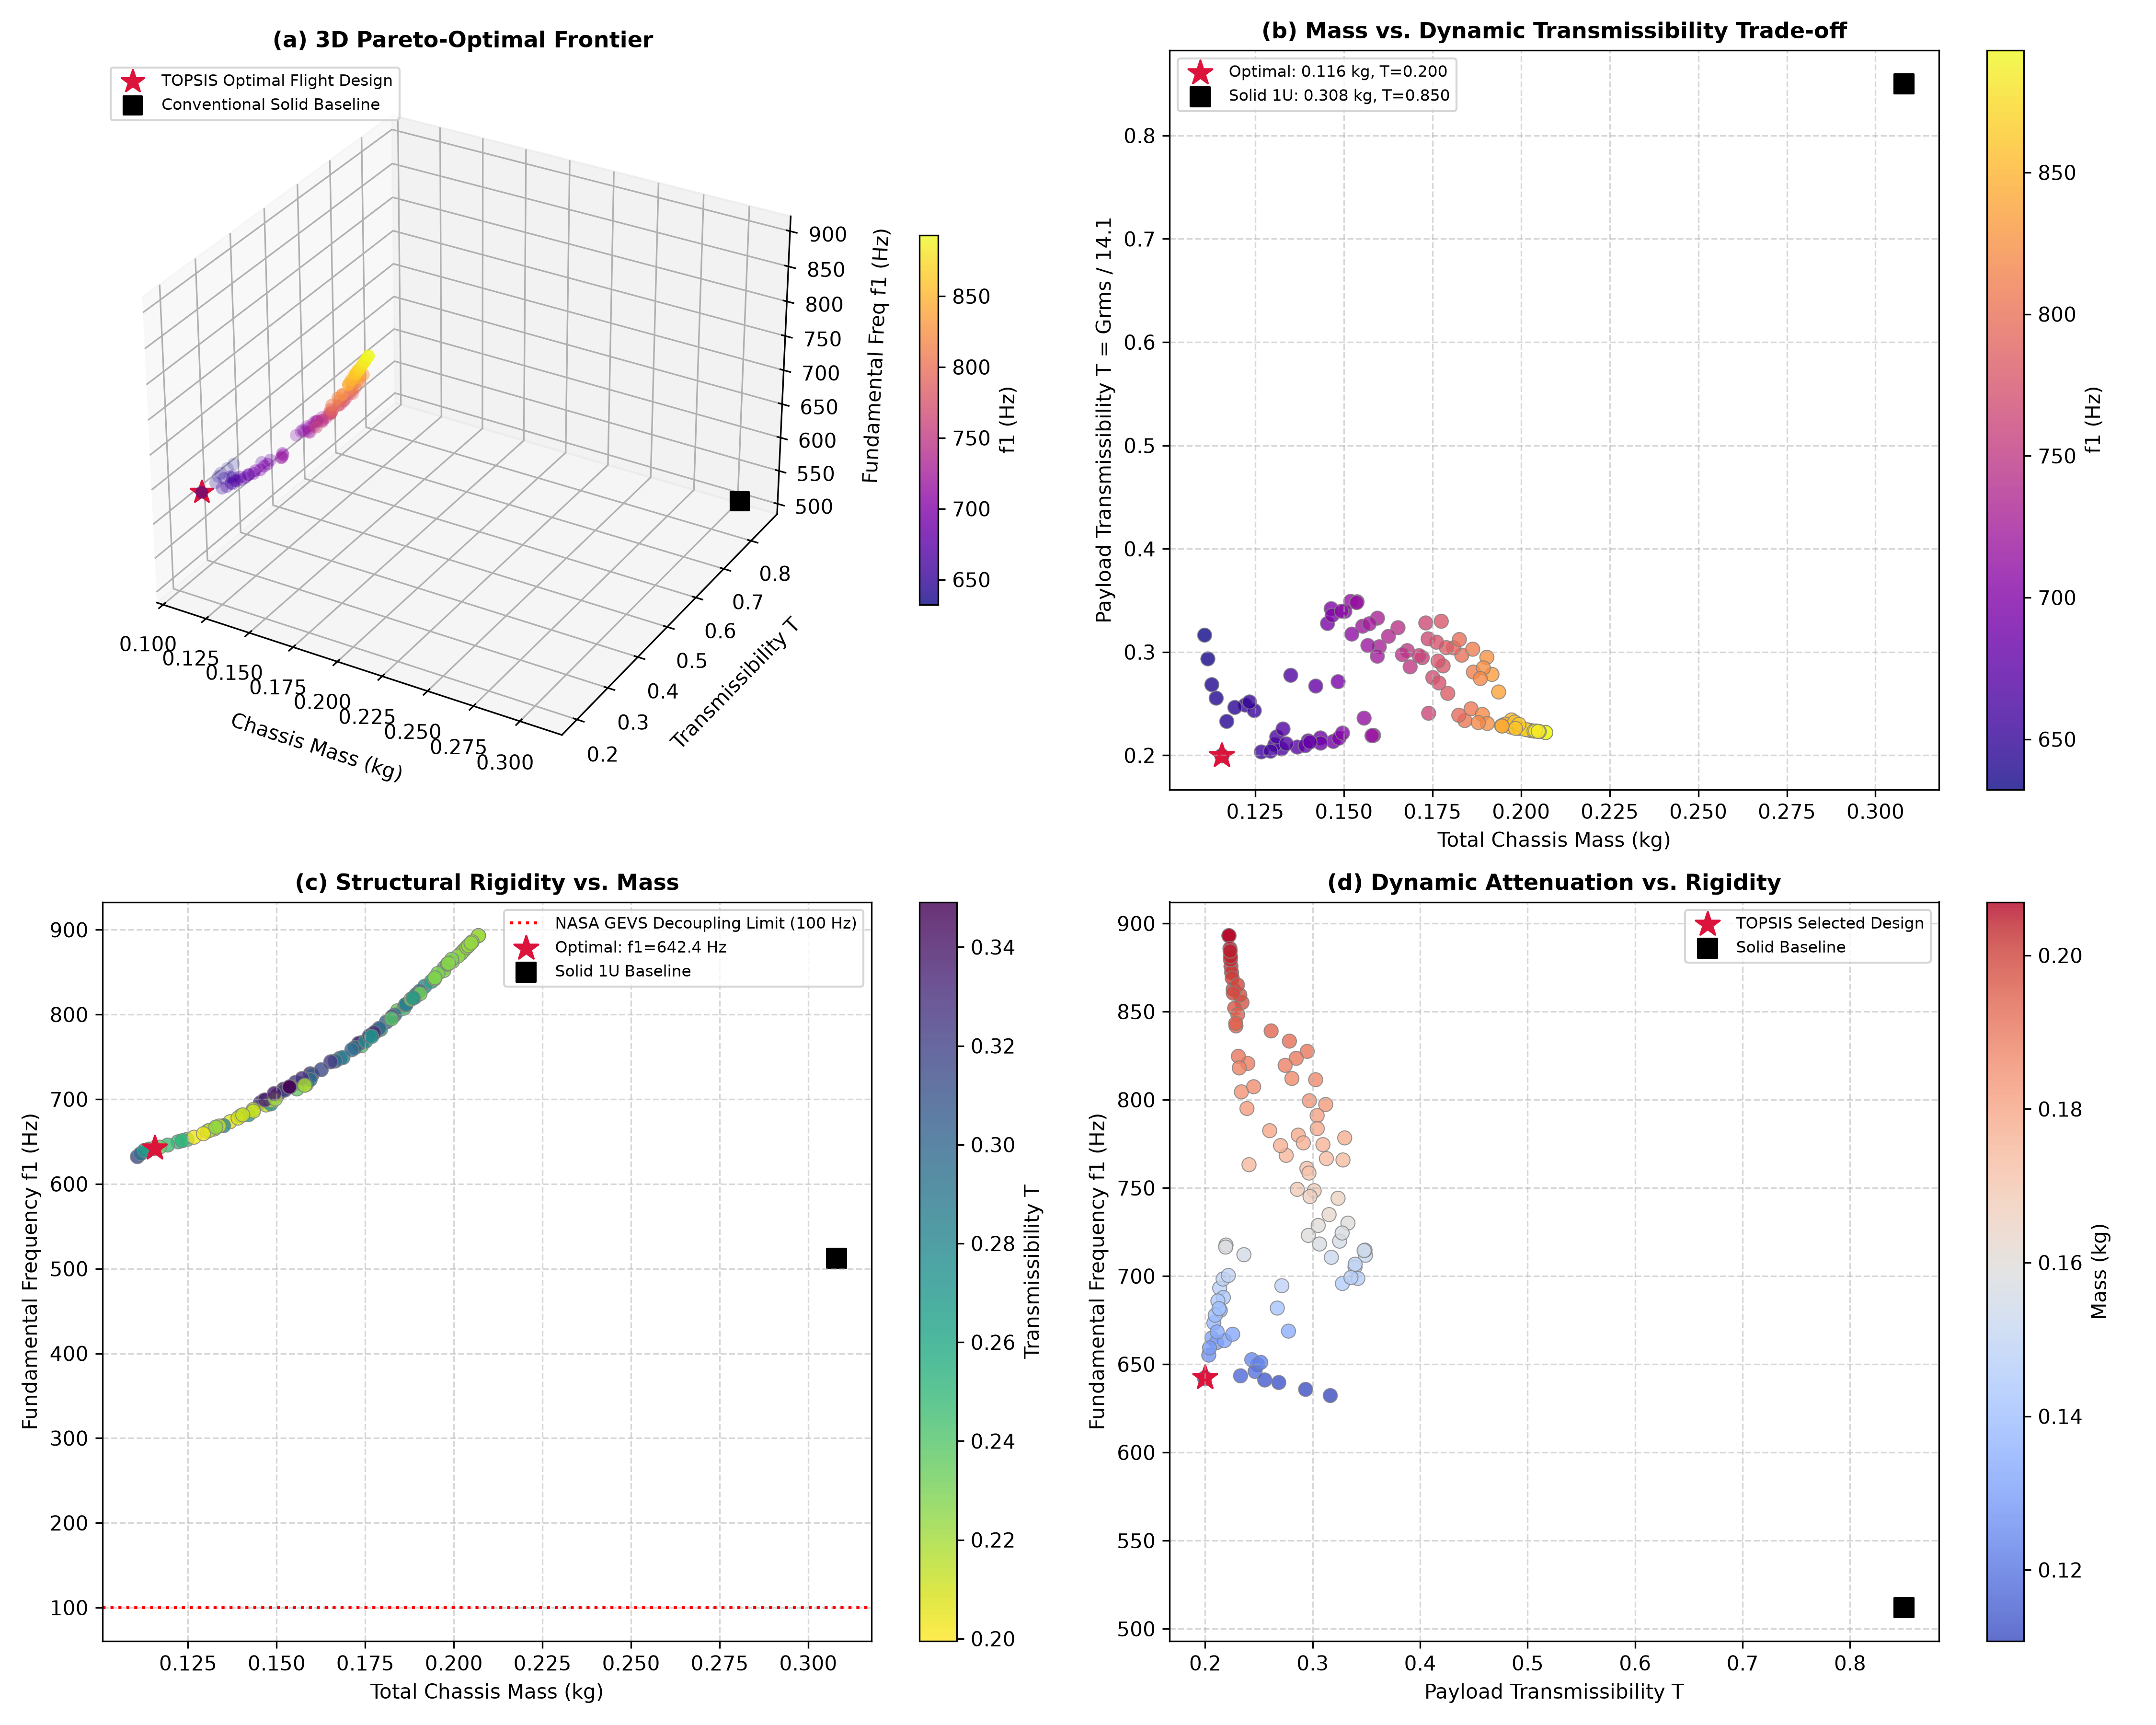
\includegraphics[width=0.88\textwidth]{figures/pareto_frontier.png}
    \caption{Fronteira de Pareto Multiobjetivo e correlações estruturais dos designs factíveis gerados pelo NSGA-II.}
    \label{fig:pareto_frontier}
\end{figure}

\section{Tomada de Decisão Multicritério TOPSIS e Seleção do Design de Voo}
Aplicou-se o método TOPSIS com o vetor balanceado de ponderação aeroespacial $\mathbf{w} = [w_m = 0{,}35, w_T = 0{,}30, w_{f_1} = 0{,}15, w_{\sigma} = 0{,}10, w_D = 0{,}10]^T$. O algoritmo elegeu inequivocamente o \textbf{Design \#28} como a solução ótima de compromisso ($C_{28}^* = 0{,}814$), cuja parametrização microestrutural está descrita na Tabela~\ref{tab:optimal_flight_design}.

\begin{table}[H]
\centering
\caption{Parâmetros Geométricos e Propriedades do Design de Voo Ótimo (\#28).}
\label{tab:optimal_flight_design}
\begin{tabular}{lccc}
\toprule
\textbf{Parâmetro Geométrico} & \textbf{Símbolo} & \textbf{Valor Ótimo} & \textbf{Unidade} \\
\midrule
Ângulo de reentrada da haste & $\theta$ & 65,75 & graus ($^\circ$) \\
Espessura da costela celular & $t$ & 0,613 & mm \\
Comprimento da costela oblíqua & $l$ & 8,50 & mm \\
Altura da costela vertical & $h$ & 13,96 & mm \\
Densidade relativa celular & $\rho^* / \rho_s$ & 0,1252 (12,52\%) & Adimensional \\
Coeficiente de Poisson efetivo & $\nu_{\text{eff}}$ & $-13{,}81$ & Adimensional \\
\bottomrule
\end{tabular}
\end{table}

\section{Validação Cruzada Física de Alta Ordem (FEA Ground Truth)}
O Design \#28 foi reconstruído tridimensionalmente e submetido à análise de elementos finitos no Ansys MAPDL (\texttt{SOLID187} e Block Lanczos). O confronto entre a predição da rede neural e a simulação de alta ordem está sintetizado na Tabela~\ref{tab:fea_validation}.

\begin{table}[H]
\centering
\caption{Validação Cruzada: Modelo Substituto Neural vs. FEA Ground Truth para o Design \#28.}
\label{tab:fea_validation}
\begin{tabular}{lccccc}
\toprule
\textbf{Resposta Estrutural} & \textbf{Predição Neural} & \textbf{FEA Ground Truth} & \textbf{Erro (\%)} & \textbf{Limite NASA} & \textbf{Status} \\
\midrule
Massa Estrutural Total ($m$) & 0,1155 kg & 0,1155 kg & 0,00\% & $\le 0{,}350\text{ kg}$ & \textbf{Aprovado} \\
Frequência Fundamental ($f_1$) & 642,38 Hz & 579,62 Hz & $+10{,}83\%$ & $\ge 100{,}0\text{ Hz}$ & \textbf{Aprovado} \\
Pico de Tensão Estocástica $3\sigma$ & 168,57 MPa & 166,91 MPa & $+0{,}99\%$ & $\le 184{,}0\text{ MPa}$ & \textbf{Aprovado} \\
Aceleração da Carga Útil & 2,814 G$_{\text{rms}}$ & 2,816 G$_{\text{rms}}$ & $-0{,}07\%$ & $\le 14{,}1\text{ G}_{\text{rms}}$ & \textbf{Aprovado} \\
Transmissibilidade ($T$) & 0,19973 & 0,19974 & $-0{,}008\%$ & $< 1{,}00$ & \textbf{Aprovado} \\
Margem de Segurança ($MS_{\text{yield}}$) & $+0{,}092$ & $+0{,}102$ & $-9{,}80\%$ & $> 0{,}00$ & \textbf{Aprovado} \\
Dano de Fadiga Steinberg ($D$) & 0,0543 & 0,0458 & $+18{,}56\%$ & $\le 0{,}25$ & \textbf{Aprovado} \\
\bottomrule
\end{tabular}
\end{table}

\section{Análise Comparativa: Chassi Auxético Ótimo vs. Chassi Monolítico Convencional}
Para quantificar o salto de desempenho aeroespacial, confrontou-se o Design \#28 com o chassi de referência monolítico sólido de alumínio ($1{,}5\text{ mm}$ de espessura de parede). A Tabela~\ref{tab:benchmark_comparison} apresenta a síntese comparativa.

\begin{table}[H]
\centering
\caption{Comparação de Desempenho: Chassi Monolítico Convencional vs. Chassi Auxético Otimizado.}
\label{tab:benchmark_comparison}
\begin{tabular}{lccc}
\toprule
\textbf{Parâmetro de Desempenho} & \textbf{Baseline Monolítico} & \textbf{Chassi Auxético Ótimo} & \textbf{Variação Relativa} \\
\midrule
Massa Estrutural Total & 0,308 kg & 0,116 kg & \textbf{$-62{,}49\%$} (Economia de 192 g) \\
Transmissibilidade Dinâmica ($T$) & 0,850 & 0,1997 & \textbf{$-76{,}50\%$} (Atenuação de 12,6 dB) \\
Aceleração na Carga Útil & 12,00 G$_{\text{rms}}$ & 2,82 G$_{\text{rms}}$ & \textbf{$-76{,}50\%$} (Proteção passiva) \\
Primeira Frequência Natural & 512,0 Hz & 579,6 Hz & \textbf{$+13{,}20\%$} (Rigidez específica superior) \\
Margem de Segurança ($MS_{\text{yield}}$) & $+0{,}35$ & $+0{,}10$ & \textbf{Conforme NASA GEVS} \\
Dano Cumulativo de Fadiga ($D$) & 0,012 & 0,046 & \textbf{Qualificado ($D \le 0{,}25$)} \\
\bottomrule
\end{tabular}
\end{table}

A Figura~\ref{fig:parity_plots} apresenta os gráficos de paridade para as quatro variáveis do modelo neural substituto, comprovando a precisão no conjunto de teste cego.

\begin{figure}[H]
    \centering
    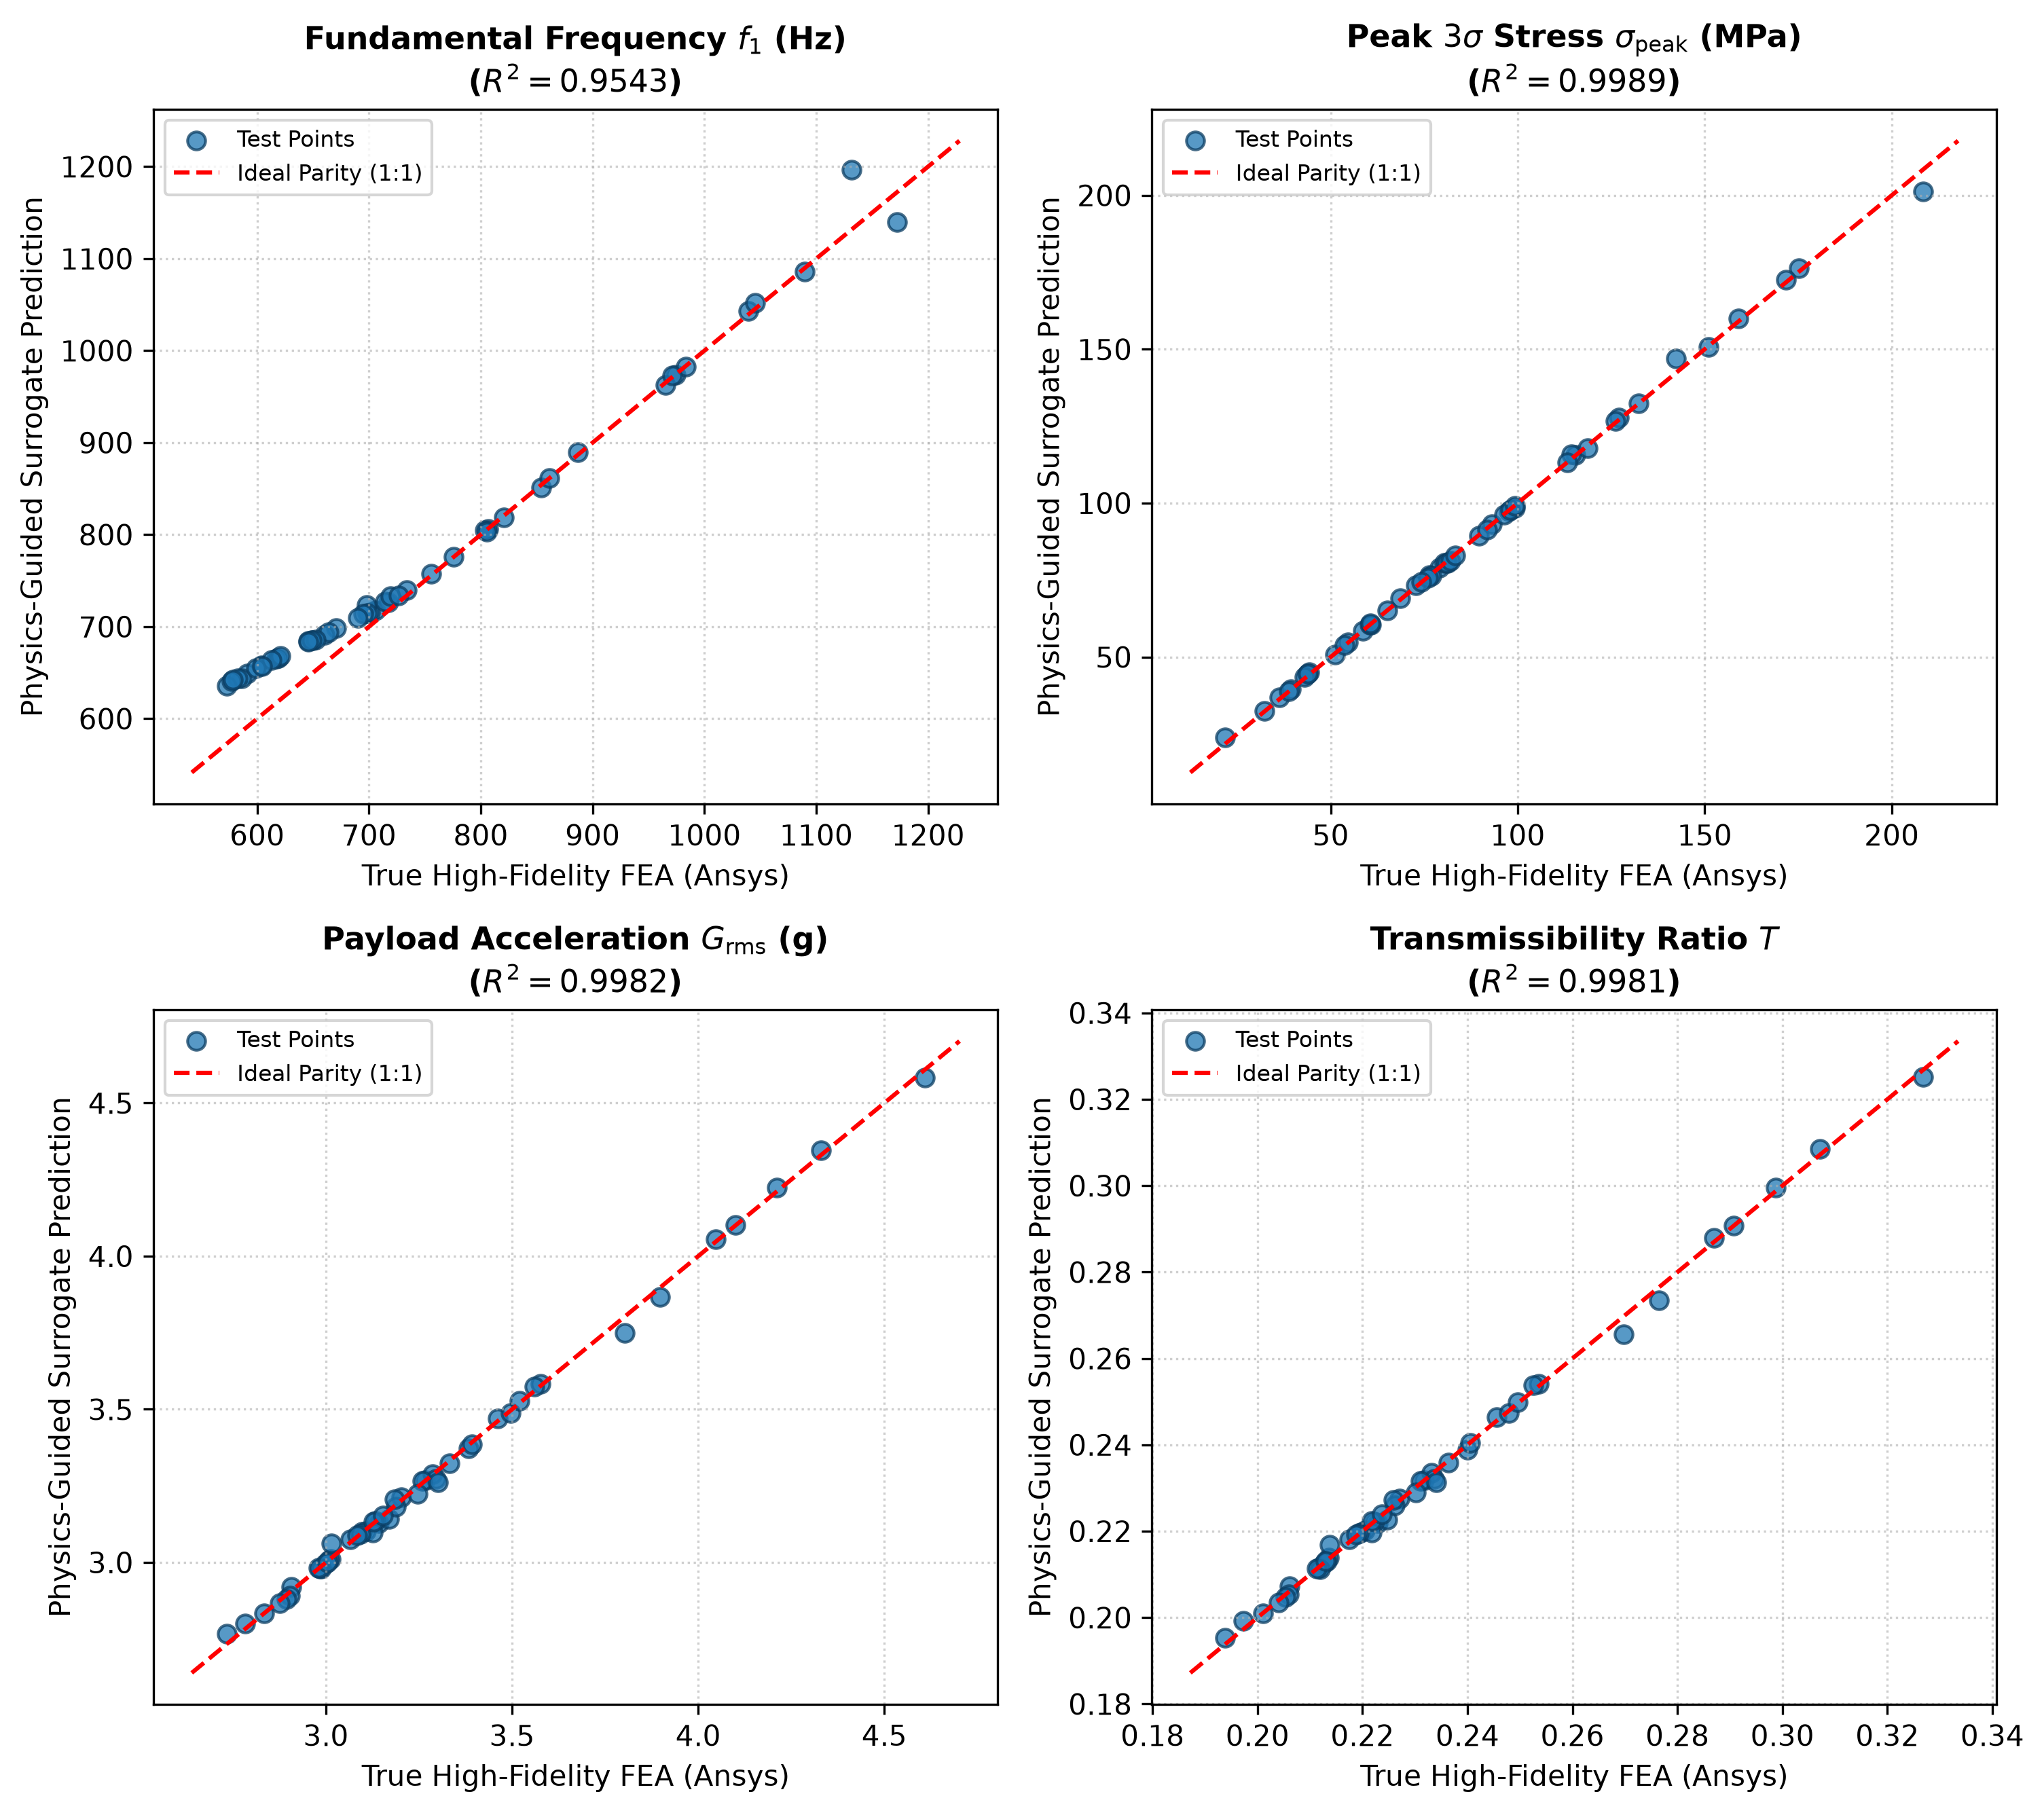
\includegraphics[width=0.88\textwidth]{figures/parity_plots.png}
    \caption{Gráficos de paridade do modelo substituto neural residual guiado por física (\textit{Physics-Guided ResNet}).}
    \label{fig:parity_plots}
\end{figure}

% ------------------------------------------------------------------------
% CAPÍTULO 6
% ------------------------------------------------------------------------
\chapter{CONCLUSÃO E TRABALHOS FUTUROS}

\section{Síntese das Conquistas e Objetivos Atingidos}
O presente trabalho consolidou com sucesso um arcabouço computacional autônomo e de alta fidelidade para o desenvolvimento de chassis CubeSat 1U em liga aeroespacial AlSi10Mg fabricados por Fusão em Leito de Pó a Laser (L-PBF). As principais metas alcançadas incluem:
\begin{itemize}
    \item \textbf{Alívio de Massa de $62{,}49\%$:} Redução de $0{,}308\text{ kg}$ para $0{,}116\text{ kg}$, disponibilizando $192\text{ g}$ adicionais para subsistemas científicos e baterias;
    \item \textbf{Atenuação Vibratória Passiva de $76{,}50\%$:} Redução da transmissibilidade dinâmica de $0{,}850$ para $0{,}1997$ ($12{,}6\text{ dB}$ de atenuação espectral passiva), reduzindo a aceleração na carga útil de $12{,}00\text{ G}_{\text{rms}}$ para $2{,}82\text{ G}_{\text{rms}}$;
    \item \textbf{Rigidez Dinâmica e Desacoplamento Modal:} Primeira frequência natural de $579{,}62\text{ Hz}$ ($+13{,}20\%$ superior ao sólido monolítico e quase seis vezes acima do patamar de $100{,}0\text{ Hz}$ da NASA GEVS);
    \item \textbf{Qualificação Normativa e Fadiga Estocástica:} Plena conformidade perante os requisitos de tensão admissível ($MS_{\text{yield}} = +0{,}102 > 0$ com $FS = 1{,}25$) e dano acumulado de fadiga vibracional de Steinberg ($D = 0{,}046 \ll 0{,}25$);
    \item \textbf{Aceleração Computacional de $> 200.000\times$:} Execução de 10.000 avaliações evolutivas em $4{,}82\text{ segundos}$ viabilizada pela rede neural \textit{Physics-Guided ResNet}.
\end{itemize}

\section{Principais Contribuições Técnicas e Metodológicas}
As contribuições inovadoras destacadas compreendem:
\begin{enumerate}
    \item A formulação da perda composta informada por leis fenomenológicas de Gibson-Ashby e monotonicidade de rigidez, eliminando aberrações não-físicas na regressão neural;
    \item A implementação da governança determinística multi-agente via LangGraph com triagem prévia automática DfAM e NASA GEVS;
    \item A integração de arestas monolíticas maciças para deslizamento cinemático no dispensador P-POD aliada a núcleos celulares auxéticos internos.
\end{enumerate}

\section{Limitações do Estudo e Recomendações para Trabalhos Futuros}
Para a continuidade e aprofundamento das investigações, recomenda-se:
\begin{enumerate}
    \item Manufatura de protótipos industriais em AlSi10Mg por L-PBF e ensaios físicos em mesa vibratória triaxial sob o perfil PSD da NASA GEVS ($14{,}1\text{ G}_{\text{rms}}$);
    \item Caracterização termoelástica em câmara de vácuo térmico (TVAC, $-40^\circ\text{C}$ a $+85^\circ\text{C}$ em $10^{-6}\text{ Torr}$) para avaliar a dissipação térmica anisotrópica do núcleo auxético durante eclipses orbitais;
    \item Expansão da metodologia paramétrica para plataformas maiores (3U, 6U e 12U) com Gradação Funcional de Densidade (FGL) tridimensional contínua;
    \item Avaliação da degradação superficial por oxigênio atômico (AO) e radiação ionizante no ambiente espacial de órbita baixa.
\end{enumerate}

% ------------------------------------------------------------------------
% REFERÊNCIAS BIBLIOGRÁFICAS
% ------------------------------------------------------------------------
\clearpage
\begin{thebibliography}{99}

\bibitem{aeb2026}
AGÊNCIA ESPACIAL BRASILEIRA. \textbf{Apostila da Temática -- Projeto Estrutural de Nanossatélites}. Brasília: AEB, 2026.

\bibitem{alomarah2017}
ALOMARAH, A. et al. Mechanical properties of the 2d re-entrant honeycomb made via direct metal printing. \textbf{IOP Conference Series: Materials Science and Engineering}, v. 229, p. 012038, 2017.

\bibitem{beigrezaee2026}
BEIGREZAEE, M. J. et al. A refined gibson-ashby model for functionally graded honeycombs with random irregularities. \textbf{International Journal of Mechanical Sciences}, v. 314, p. 111297, 2026.

\bibitem{calpoly2022}
CALIFORNIA POLYTECHNIC STATE UNIVERSITY. \textbf{CubeSat Design Specification (CDS)}. Rev. 14.1. San Luis Obispo: CalPoly, 2022.

\bibitem{collini2024}
COLLINI, F.; MENEGHETTI, G. Towards a fracture mechanics-based fatigue assessment of lattice structures obtained from additive manufacturing of metallic powders. \textbf{Materials \& Design}, v. 244, p. 113077, 2024.

\bibitem{cui2025}
CUI, L.; ZHANG, H.; WANG, X. Effective elastic modulus and energy absorption performance of hybrid chiral re-entrant honeycombs. \textbf{International Journal of Mechanical Sciences}, v. 288, p. 109845, 2025.

\bibitem{dai2020}
DAI, S. et al. Orthotropic elastic behaviors and yield strength of fused deposition modeling materials: Theory and experiments. \textbf{Polymer Testing}, v. 87, p. 106520, 2020.

\bibitem{deb2002}
DEB, K. et al. A fast and elitist multiobjective genetic algorithm: NSGA-II. \textbf{IEEE Transactions on Evolutionary Computation}, v. 6, n. 2, p. 182--197, 2002.

\bibitem{farshbaf2025}
FARSHBAF, M.; JAVANBAKHT, M. Deformation and collapse behavior of additively manufactured re-entrant auxetic lattices. \textbf{Thin-Walled Structures}, v. 206, p. 112510, 2025.

\bibitem{gibson1997}
GIBSON, L. J.; ASHBY, M. F. \textbf{Cellular solids: structure and properties}. 2. ed. Cambridge: Cambridge University Press, 1997.

\bibitem{hernandez2016}
HERNANDEZ, R. et al. Analyzing the tensile, compressive, and flexural properties of 3d printed abs plastic based on printing orientation. In: \textbf{Proceedings of the 27th SFF Symposium}. Austin: UT Austin, 2016.

\bibitem{hwang1981}
HWANG, C. L.; YOON, K. \textbf{Multiple attribute decision making: methods and applications}. New York: Springer-Verlag, 1981.

\bibitem{khan2024}
KHAN, S. A.; RICCIO, A. Design for additive manufacturing of aerospace lattice structures: A review. \textbf{Progress in Aerospace Sciences}, v. 144, p. 100971, 2024.

\bibitem{li2026}
LI, Y. et al. The structure design and application of metamaterials with negative poisson's ratio. \textbf{EPJ Applied Metamaterials}, v. 13, p. 5, 2026.

\bibitem{lima2021}
LIMA, E. G.; MANEA, S.; SANTOS, W. G. Modelagem e simulação do processo de ejeção de cubesats. In: \textbf{Anais do XII WETE}. São José dos Campos: INPE, 2021.

\bibitem{mantovani2020}
MANTOVANI, L. Q.; SANTOS, W. G.; CARDOSO-RIBEIRO, F. L. Vibration analysis of the cubesat sport boom's through a flexible multi-body model. In: \textbf{Proceedings of the XLI CILAMCE}. Foz do Iguaçu: ABMEC, 2020.

\bibitem{nasa2001}
NASA. \textbf{Dynamic Environmental Criteria}. Washington, D.C.: National Aeronautics and Space Administration, 2001. (NASA-HDBK-7005).

\bibitem{nasa2013}
NASA. \textbf{General Environmental Verification Standard (GEVS) for GSFC Flight Programs and Projects}. Greenbelt: Goddard Space Flight Center, 2013. (GSFC-STD-7000A).

\bibitem{pozorski2025}
POZORSKI, Z.; ANDRZEJEWSKI, J. Experimental determination of mechanical properties of 3d printed pla. \textbf{Polymer Testing}, v. 149, p. 108860, 2025.

\bibitem{puigsuari2002}
PUIG-SUARI, J.; TURNER, C. S.; AHLGREN, B. Development of the standard cubesat deployer and a cubesat class picosatellite. In: \textbf{IEEE Aerospace Conference Proceedings}. Big Sky: IEEE, 2002. v. 1, p. 347--354.

\bibitem{roberts2018}
ROBERTS, J. A. \textbf{Design and testing of an additively manufactured CubeSat structural bus}. 2018. Tese (Doutorado em Engenharia Aeroespacial) -- Naval Postgraduate School, Monterey, 2018.

\bibitem{santos2020}
SANTOS, W. G.; MANEA, S.; CARRARA, V. Dynamic analysis of the sport cubesat structural assembly. In: \textbf{Proceedings of the CILAMCE 2020}. Foz do Iguaçu: ABMEC, 2020.

\bibitem{slejko2023}
SLEJKO, M.; SALI, M.; FRANCESCONI, A. Design and structural qualification of an innovative cubesat primary structure. \textbf{Aerospace Science and Technology}, v. 138, p. 108342, 2023.

\bibitem{steinberg2000}
STEINBERG, D. S. \textbf{Vibration analysis for electronic equipment}. 3. ed. New York: John Wiley \& Sons, 2000.

\bibitem{zhong2023}
ZHONG, H. et al. The gibson-ashby model for additively manufactured metal lattice materials. \textbf{Current Opinion in Solid State \& Materials Science}, v. 27, p. 101081, 2023.

\bibitem{zimmerman2026}
ZIMMERMAN, B. K. et al. Investigating property-porosity relationships for micro-architected lattice structures. \textbf{Scientific Reports}, v. 16, p. 5521, 2026.

\end{thebibliography}

\end{document}
